\documentclass{beamer}
\usepackage{packages}
\graphicspath{ {./imgs/}{../imgs/} }

% \usetheme{AnnArbor}
\usetheme{Warsaw}
\usecolortheme{beaver}
\useoutertheme{miniframes}
\setbeamertemplate{headline}{}
\setbeamertemplate{title page}[default][rounded=true]
\setbeamertemplate{frametitle}[default][colsep=0bp,rounded=false,shadow=false]
\setbeamercolor{frametitle}{bg=beaverdarkred,fg=white}
\setbeamercolor{framesubtitle}{bg=darkunq}
\setbeamercolor{title}{fg=beaverdarkred}
\setbeamercolor{subtitle}{fg=beaverdarkred}
\setbeamercolor{author in head/foot}{fg=beaverdarkred,bg=darkgrey}
\setbeamertemplate{footline}
{
    \leavevmode%
    \hbox{%
    \begin{beamercolorbox}[wd=1\paperwidth,ht=2.25ex,dp=1ex,center]{title in head/foot}%
        \usebeamerfont{title in head/foot}\insertshortauthor\insertshorttitle\hspace*{2em}
    \end{beamercolorbox}}%
    \vskip0pt%
}
\setbeamertemplate{itemize item}[triangle]
\setitemize{label=\usebeamerfont*{itemize item}%
  \usebeamercolor[fg]{itemize item}
  \usebeamertemplate{itemize item}}




\title[\texttt{ UNQ -> TIP -> MQL}]{Mumuki Query Learning}
\subtitle{\emph{Un Runner de SQL para el Proyecto Mumuki}}

\titlegraphic{
    
\includegraphics[width=.4\textwidth]{logo-unq}
}

\author[\texttt{Leandro Di Lorenzo ::}]
{
    Leandro~Di~Lorenzo \\
    \textbf{Coordinador:} Ing. Fernando Dodino
    % \vspace{-1em}
}


\institute[TIP - UNQ]
{
   \textsc{
       \small{Tecnicatura en Programación Informática}
   }
}

\date[jul 2017]{8 de Julio, 2017}


\makeatletter
    \newenvironment{withoutheadline}{
        \setbeamertemplate{headline}[default]
        \def\beamer@entrycode{\vspace*{-\headheight}}
    }{}
\makeatother



\begin{document}


%%
%% Carátula
%%
\begin{frame}[plain]
    \vspace{2em}
    \titlepage
    \vspace{-2em}
    \begin{figure}[h]
        
\includegraphics[scale=1]{logo-unq}
    \end{figure}
\end{frame}


%%
%% Idea: MQL
%%
\begin{frame}{Idea: MQL}
    \begin{figure}[h]
        
\includegraphics[scale=1]{logo-mql}
    \end{figure}
\end{frame}


%%
%% Proyecto Mumuki
%%
\begin{frame}{Proyecto Mumuki}
    \begin{figure}[h]
        
\includegraphics[width=1\textwidth]{proyecto-mumuki}
    \end{figure}
\end{frame}


%%
%% Un poco de data...
%%
\begin{frame}{Un poco de data...}
    \begin{itemize}%[<+->]
        \item Mumuki es una plataforma educativa para la enseñanza de programación, y es \textit{Open Source}.
        \item Se puede utilizar de forma autodidacta o como aula virtual con seguimiento.
        \item Es desarrollada y mantenida por estudiantes y docentes de varias universidades públicas, incluída la UNQ.
        \item Está siendo utilizada en diferentes entidades educativas del país.
        \item Tiene un enfoque didáctico con fuerte incapié en los conceptos por sobre las tecnologías.
    \end{itemize}
\end{frame}


%%
%% Mumuki :: Ejercicios
%%
\begin{frame}{Mumuki :: Ejercicios}
    \begin{figure}[h]
        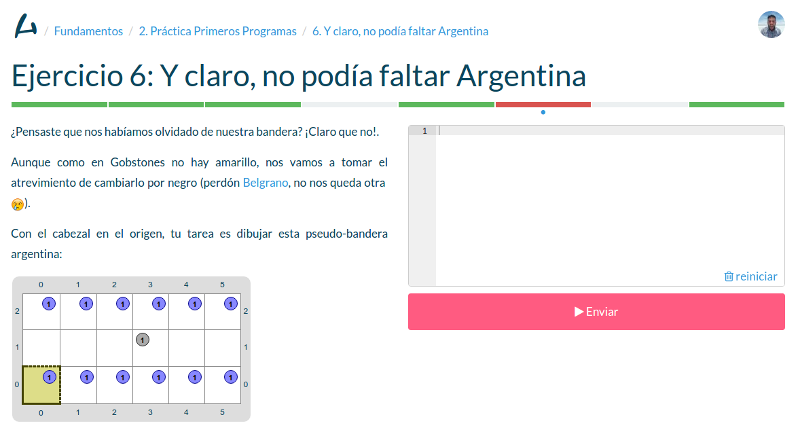
\includegraphics[width=1\textwidth]{gobstones-exercise}
    \end{figure}
\end{frame}

%%
%% Mumuki :: Corrección Automatizada
%%
\begin{frame}{Mumuki :: Corrección Automatizada}
    \begin{figure}[h]
        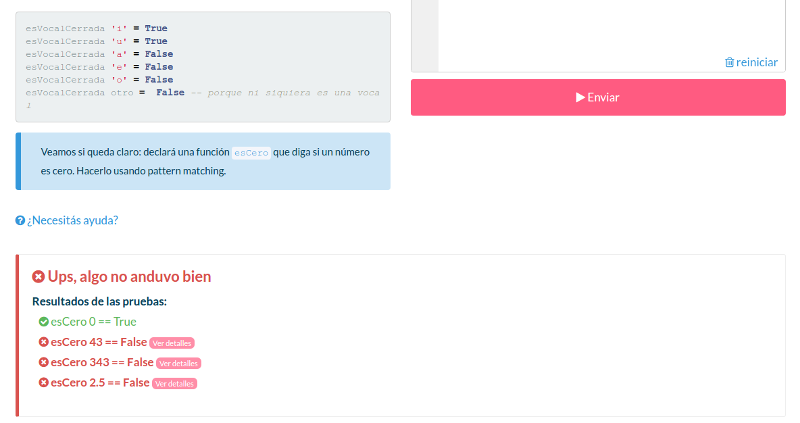
\includegraphics[width=1\textwidth]{haskell-ups}
    \end{figure}
\end{frame}

%%
%% Mumuki :: Seguimiento
%%
\begin{frame}{Mumuki :: Seguimiento}
    \begin{figure}[h]
        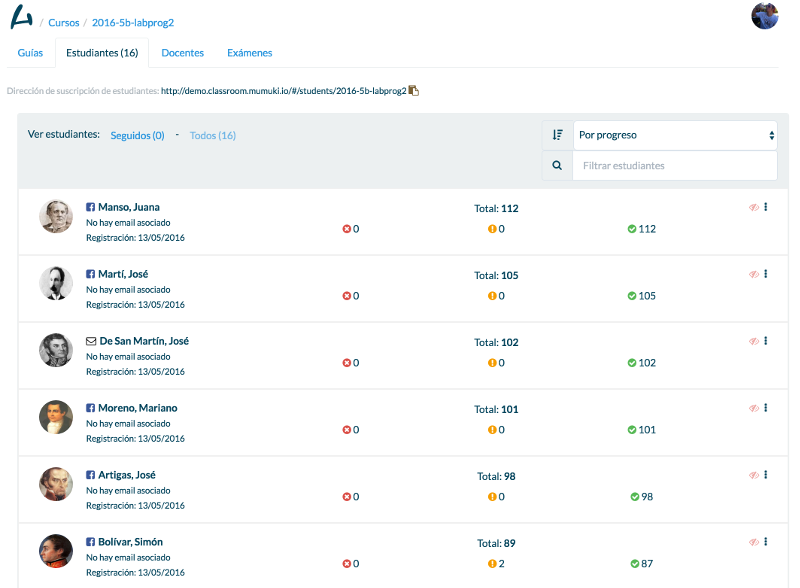
\includegraphics[width=1\textwidth]{classroom-students}
    \end{figure}
\end{frame}


%%
%% Mumuki :: Versionado
%%
\begin{frame}{Mumuki :: Versionado}
    \begin{figure}[h]
        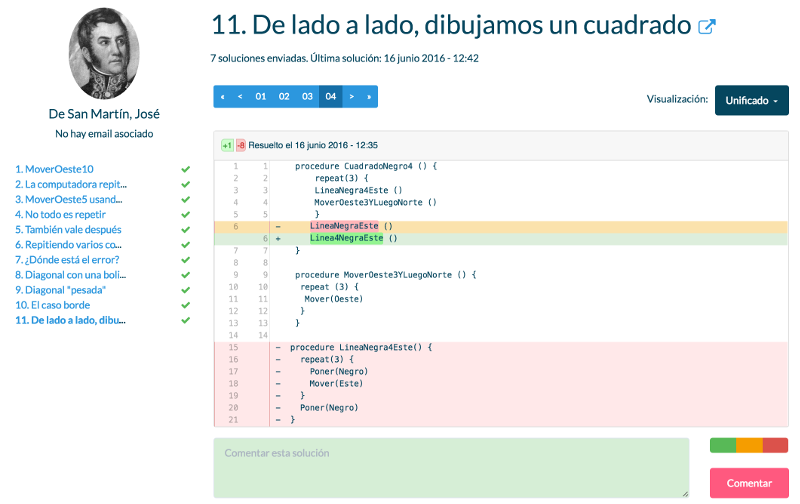
\includegraphics[width=1\textwidth]{classroom-student-detail}
    \end{figure}
\end{frame}


%%
%% Mumuki :: Contenido Personalizable
%%
\begin{frame}{Mumuki :: Contenido Personalizable}
    \begin{figure}[h]
        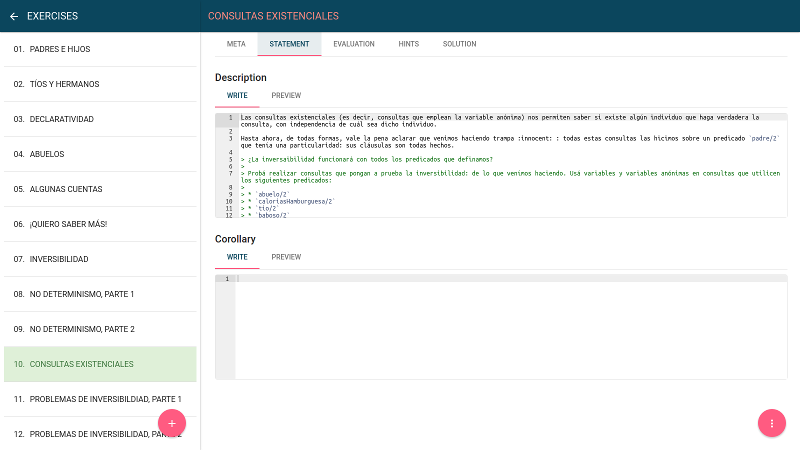
\includegraphics[width=1\textwidth]{editor}
    \end{figure}
\end{frame}


%%
%% Mumuki :: Contenido Actual
%%
\begin{frame}{Mumuki :: Contenido Actual}
    \begin{figure}[h]
        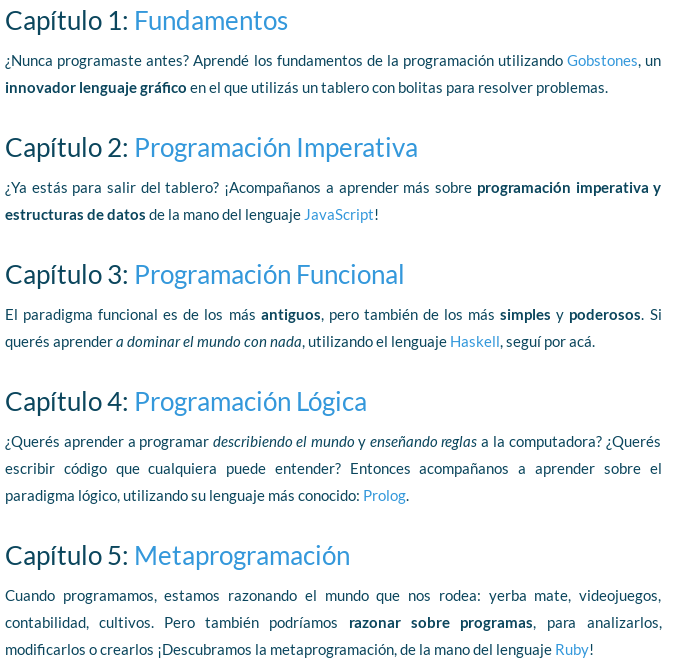
\includegraphics[width=.85\textheight]{contenido}
    \end{figure}
\end{frame}


%%
%% Mumuki Query Learning :: Objetivos
%%
\begin{frame}{Mumuki Query Learning :: Objetivos}

    Proveer a los docentes de \textit{Bases de Datos} una herramienta para:

    \begin{itemize}
        \item Mejorar la didáctica en la enseñanza de conceptos de SQL
        \item Facilitar el seguimiento del aprendizaje de los alumnos
        \item Contar con mejores elementos de evaluación
    \end{itemize}

    \vspace{1em}

    Proveer a los alumnos una herramienta para:

    \begin{itemize}
        \item Comprender mejor los conceptos recibidos
        \item Recibir feedback de forma temprana
        \item Poder analizar por su cuenta los fallos obtenidos para poder aprender de ellos
        \item Analizar su propio progreso visualizando los pasos dados hasta la resolución de los problemas
    \end{itemize}
\end{frame}

%%
%% Consecuencias Deseadas
%%
\begin{frame}{MQL :: Consecuencias Deseadas}

    \begin{itemize}
        \setlength\itemsep{1em}
        \item Aportar al crecimiento del \textit{Proyecto Mumuki} con una nueva tecnología de aprendizaje.
        \item Ayudar a todo programador que desee mejorar su capacidad y calidad en
        relación al uso de las bases de datos relaciones.
        \item Dejar abierta la posibilidad de extensión hacia:
        \vspace{.4em}
        \begin{itemize}
            \setlength\itemsep{.5em}
            \item Álgebra Relacional
            \item Bases de datos no relaciones (MongoDB, Neo4j, Redis, etc...)
        \end{itemize}
    \end{itemize}

\end{frame}


%%
%% Herramientas a Implementar
%%
\begin{frame}{MQL :: Herramientas a Implementar}
    \begin{itemize}%[<+->]
        \setlength\itemsep{1em}
        \item Docker container con PostgreSQL o SQLite
        \item Runner de SQL en Ruby que permita:
        \vspace{.4em}
        \begin{itemize}
            \setlength\itemsep{.5em}
            \item Obtener y ejecutar el código SQL recibido
            \item Validar resultados obtenidos contra esperados
            \item Analizar sintaxis para exponer buenas prácticas de código
        \end{itemize}
        \item Classroom con set de ejercicios
    \end{itemize}
\end{frame}


%%
%% Mumuki :: Organizaciones que la utilizan
%%
\begin{frame}{Mumuki :: Organizaciones que la utilizan}
    \begin{figure}[h]
        
\includegraphics[width=1\textwidth]{organizaciones}
    \end{figure}
\end{frame}


%%
%% Algunos Links
%%
\begin{frame}{Algunos Links}
    \begin{itemize}%[<+->]
        \setlength\itemsep{.7em}
        \item Proyecto Mumuki: \url{http://www.mumuki.org/}
        \item Plataforma: \url{https://mumuki.io/}
        \item Código en GitHub: \url{https://github.com/mumuki}
        \item Nota en Télam: \url{http://www.telam.com.ar/notas/201703/183460-mumuki-plataforma-gratuita-programacion\\-aprendizaje-ensenanza-software.html}
        \item PostgreSQL: \url{https://www.postgresql.org/}
        \item SQLite: \url{https://www.sqlite.org/}
        \item Docker: \url{https://www.docker.com/}
    \end{itemize}
\end{frame}


%%
%% Gracias :: Preguntas
%%
\begin{frame}[plain]
    \begin{center}
        \begin{figure}[h]
            
\includegraphics[scale=.7]{questions}
        \end{figure}
        \vspace{2em}
        \Large{¿Preguntas, ideas, comentarios?}
    \end{center}
\end{frame}

\end{document}
